\documentclass{standalone}
\usepackage{tikz}
\usetikzlibrary{patterns, positioning}


\begin{document}
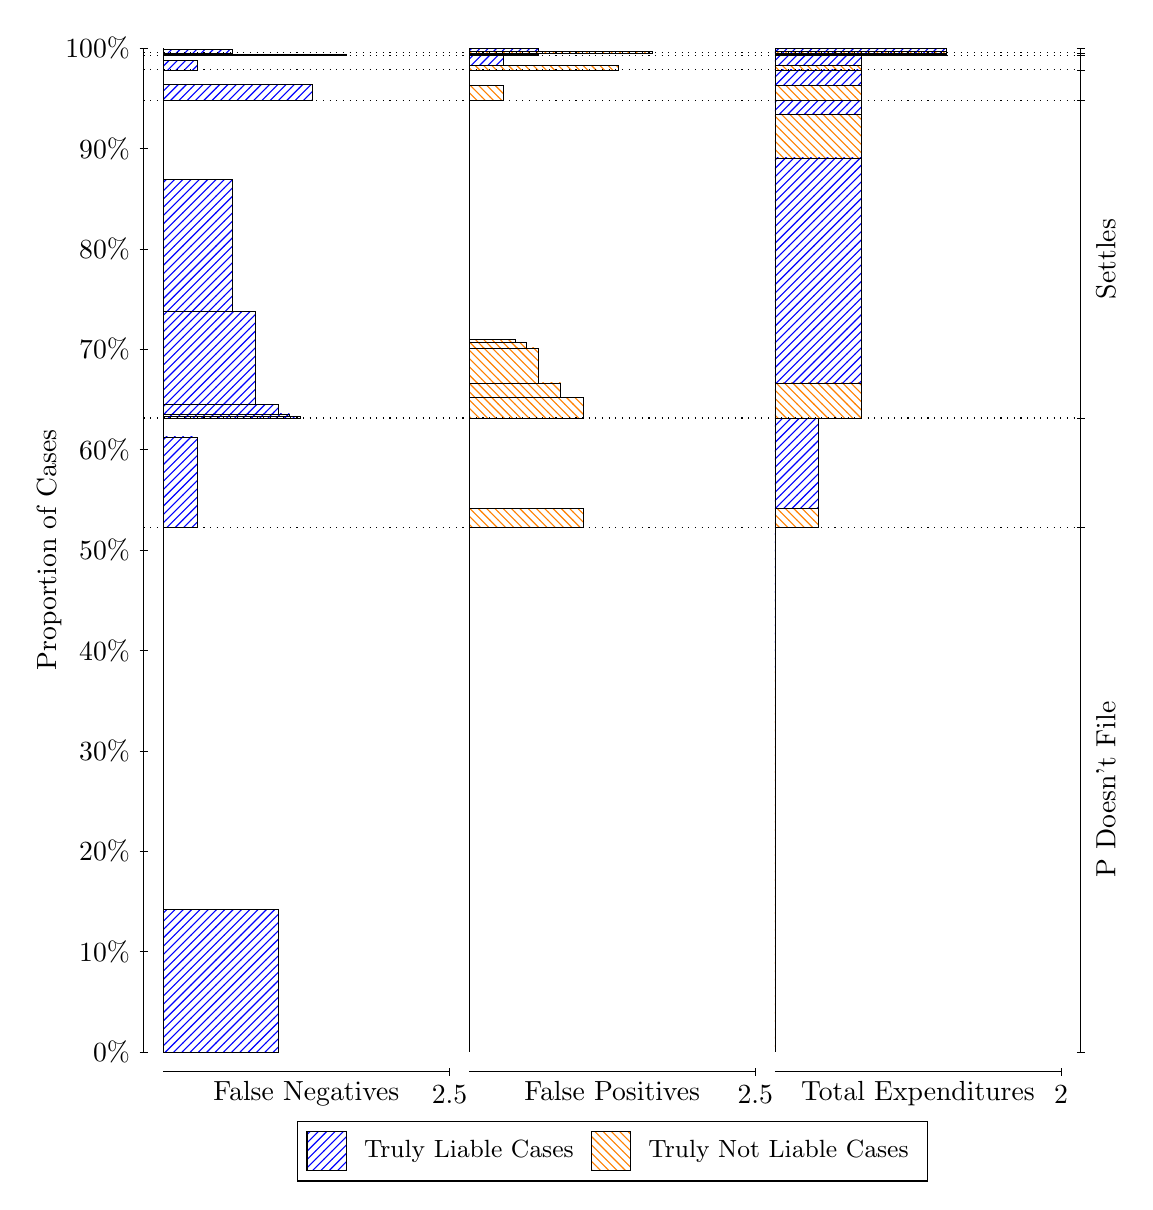
\begin{tikzpicture}
\draw[black, very thin] (1.5,1.75) -- (1.5,14.5);
\node[rotate=90, text=black, anchor=center] at (0.3, 8.125) {Proportion of Cases};
\draw[black, very thin] (1.45,1.75) -- (1.55,1.75);
\node[text=black, anchor=east] at (1.45, 1.75) {0\%};
\draw[black, very thin] (1.45,3.025) -- (1.55,3.025);
\node[text=black, anchor=east] at (1.45, 3.025) {10\%};
\draw[black, very thin] (1.45,4.3) -- (1.55,4.3);
\node[text=black, anchor=east] at (1.45, 4.3) {20\%};
\draw[black, very thin] (1.45,5.575) -- (1.55,5.575);
\node[text=black, anchor=east] at (1.45, 5.575) {30\%};
\draw[black, very thin] (1.45,6.85) -- (1.55,6.85);
\node[text=black, anchor=east] at (1.45, 6.85) {40\%};
\draw[black, very thin] (1.45,8.125) -- (1.55,8.125);
\node[text=black, anchor=east] at (1.45, 8.125) {50\%};
\draw[black, very thin] (1.45,9.4) -- (1.55,9.4);
\node[text=black, anchor=east] at (1.45, 9.4) {60\%};
\draw[black, very thin] (1.45,10.675) -- (1.55,10.675);
\node[text=black, anchor=east] at (1.45, 10.675) {70\%};
\draw[black, very thin] (1.45,11.95) -- (1.55,11.95);
\node[text=black, anchor=east] at (1.45, 11.95) {80\%};
\draw[black, very thin] (1.45,13.225) -- (1.55,13.225);
\node[text=black, anchor=east] at (1.45, 13.225) {90\%};
\draw[black, very thin] (1.45,14.5) -- (1.55,14.5);
\node[text=black, anchor=east] at (1.45, 14.5) {100\%};

\draw[black, very thin] (13.4,1.75) -- (13.4,14.5);
\draw[black, very thin] (13.35,1.75) -- (13.45,1.75);
\node[anchor=west] at (13.35, 1.75) {};
\draw[black, very thin] (13.35,8.4151) -- (13.45,8.4151);
\node[anchor=west] at (13.35, 8.4151) {};
\draw[black, very thin] (13.35,9.801) -- (13.45,9.801);
\node[anchor=west] at (13.35, 9.801) {};
\draw[black, very thin] (13.35,13.838) -- (13.45,13.838);
\node[anchor=west] at (13.35, 13.838) {};
\draw[black, very thin] (13.35,14.223) -- (13.45,14.223);
\node[anchor=west] at (13.35, 14.223) {};
\draw[black, very thin] (13.35,14.404) -- (13.45,14.404);
\node[anchor=west] at (13.35, 14.404) {};
\draw[black, very thin] (13.35,14.439) -- (13.45,14.439);
\node[anchor=west] at (13.35, 14.439) {};
\draw[black, very thin] (13.35,14.5) -- (13.45,14.5);
\node[anchor=west] at (13.35, 14.5) {};

\draw[black, very thin, pattern color=blue, pattern=north east lines] (1.75,1.75) rectangle (3.2033,3.5616);
\draw[black, very thin, pattern color=orange, pattern=north west lines] (1.75,3.5616) rectangle (1.75,8.4151);
\draw[black, very thin, pattern color=blue, pattern=north east lines] (1.75,8.4151) rectangle (2.186,9.5612);
\draw[black, very thin, pattern color=orange, pattern=north west lines] (1.75,9.5612) rectangle (1.75,9.801);
\draw[black, very thin, pattern color=blue, pattern=north east lines] (1.75,9.801) rectangle (3.494,9.8186);
\draw[black, very thin, pattern color=blue, pattern=north east lines] (1.75,9.8186) rectangle (3.3487,9.8546);
\draw[black, very thin, pattern color=blue, pattern=north east lines] (1.75,9.8546) rectangle (3.2033,9.9748);
\draw[black, very thin, pattern color=blue, pattern=north east lines] (1.75,9.9748) rectangle (2.9127,11.153);
\draw[black, very thin, pattern color=blue, pattern=north east lines] (1.75,11.153) rectangle (2.622,12.835);
\draw[black, very thin, pattern color=orange, pattern=north west lines] (1.75,12.835) rectangle (1.75,13.838);
\draw[black, very thin, pattern color=blue, pattern=north east lines] (1.75,13.838) rectangle (3.6393,14.037);
\draw[black, very thin, pattern color=orange, pattern=north west lines] (1.75,14.037) rectangle (1.75,14.223);
\draw[black, very thin, pattern color=blue, pattern=north east lines] (1.75,14.223) rectangle (2.186,14.346);
\draw[black, very thin, pattern color=orange, pattern=north west lines] (1.75,14.346) rectangle (1.75,14.404);
\draw[black, very thin, pattern color=blue, pattern=north east lines] (1.75,14.404) rectangle (4.0753,14.419);
\draw[black, very thin, pattern color=orange, pattern=north west lines] (1.75,14.419) rectangle (1.75,14.439);
\draw[black, very thin, pattern color=blue, pattern=north east lines] (1.75,14.439) rectangle (2.622,14.485);
\draw[black, very thin, pattern color=orange, pattern=north west lines] (1.75,14.485) rectangle (1.75,14.5);
\draw[black, very thin, pattern color=orange, pattern=north west lines] (5.6333,1.75) rectangle (5.6333,6.6034);
\draw[black, very thin, pattern color=blue, pattern=north east lines] (5.6333,6.6034) rectangle (5.6333,8.4151);
\draw[black, very thin, pattern color=orange, pattern=north west lines] (5.6333,8.4151) rectangle (7.0867,8.6549);
\draw[black, very thin, pattern color=blue, pattern=north east lines] (5.6333,8.6549) rectangle (5.6333,9.801);
\draw[black, very thin, pattern color=orange, pattern=north west lines] (5.6333,9.801) rectangle (7.0867,10.063);
\draw[black, very thin, pattern color=orange, pattern=north west lines] (5.6333,10.063) rectangle (6.796,10.246);
\draw[black, very thin, pattern color=orange, pattern=north west lines] (5.6333,10.246) rectangle (6.5053,10.692);
\draw[black, very thin, pattern color=orange, pattern=north west lines] (5.6333,10.692) rectangle (6.36,10.757);
\draw[black, very thin, pattern color=orange, pattern=north west lines] (5.6333,10.757) rectangle (6.2147,10.804);
\draw[black, very thin, pattern color=blue, pattern=north east lines] (5.6333,10.804) rectangle (5.6333,13.838);
\draw[black, very thin, pattern color=orange, pattern=north west lines] (5.6333,13.838) rectangle (6.0693,14.024);
\draw[black, very thin, pattern color=blue, pattern=north east lines] (5.6333,14.024) rectangle (5.6333,14.223);
\draw[black, very thin, pattern color=orange, pattern=north west lines] (5.6333,14.223) rectangle (7.5227,14.281);
\draw[black, very thin, pattern color=blue, pattern=north east lines] (5.6333,14.281) rectangle (6.0693,14.404);
\draw[black, very thin, pattern color=orange, pattern=north west lines] (5.6333,14.404) rectangle (6.5053,14.424);
\draw[black, very thin, pattern color=blue, pattern=north east lines] (5.6333,14.424) rectangle (5.6333,14.439);
\draw[black, very thin, pattern color=orange, pattern=north west lines] (5.6333,14.439) rectangle (7.9587,14.454);
\draw[black, very thin, pattern color=blue, pattern=north east lines] (5.6333,14.454) rectangle (6.5053,14.5);
\draw[black, very thin, pattern color=orange, pattern=north west lines] (9.5167,1.75) rectangle (9.5167,6.6034);
\draw[black, very thin, pattern color=blue, pattern=north east lines] (9.5167,6.6034) rectangle (9.5167,8.4151);
\draw[black, very thin, pattern color=orange, pattern=north west lines] (9.5167,8.4151) rectangle (10.062,8.6549);
\draw[black, very thin, pattern color=blue, pattern=north east lines] (9.5167,8.6549) rectangle (10.062,9.801);
\draw[black, very thin, pattern color=orange, pattern=north west lines] (9.5167,9.801) rectangle (10.607,10.246);
\draw[black, very thin, pattern color=blue, pattern=north east lines] (9.5167,10.246) rectangle (10.607,13.106);
\draw[black, very thin, pattern color=orange, pattern=north west lines] (9.5167,13.106) rectangle (10.607,13.665);
\draw[black, very thin, pattern color=blue, pattern=north east lines] (9.5167,13.665) rectangle (10.607,13.838);
\draw[black, very thin, pattern color=orange, pattern=north west lines] (9.5167,13.838) rectangle (10.607,14.024);
\draw[black, very thin, pattern color=blue, pattern=north east lines] (9.5167,14.024) rectangle (10.607,14.223);
\draw[black, very thin, pattern color=orange, pattern=north west lines] (9.5167,14.223) rectangle (10.607,14.281);
\draw[black, very thin, pattern color=blue, pattern=north east lines] (9.5167,14.281) rectangle (10.607,14.404);
\draw[black, very thin, pattern color=orange, pattern=north west lines] (9.5167,14.404) rectangle (11.697,14.424);
\draw[black, very thin, pattern color=blue, pattern=north east lines] (9.5167,14.424) rectangle (11.697,14.439);
\draw[black, very thin, pattern color=orange, pattern=north west lines] (9.5167,14.439) rectangle (11.697,14.454);
\draw[black, very thin, pattern color=blue, pattern=north east lines] (9.5167,14.454) rectangle (11.697,14.5);
\draw[black, dotted] (1.5,8.4151) -- (13.4,8.4151);
\draw[black, dotted] (1.5,9.801) -- (13.4,9.801);
\draw[black, dotted] (1.5,13.838) -- (13.4,13.838);
\draw[black, dotted] (1.5,14.223) -- (13.4,14.223);
\draw[black, dotted] (1.5,14.404) -- (13.4,14.404);
\draw[black, dotted] (1.5,14.439) -- (13.4,14.439);
\draw[black, very thin] (1.75,1.5) -- (5.3833,1.5);
\node[text=black, anchor=north] at (3.5667, 1.5) {False Negatives};
\draw[black, very thin] (5.3833,1.45) -- (5.3833,1.55);
\node[text=black, anchor=north] at (5.3833, 1.45) {2.5};

\draw[black, very thin] (5.6333,1.5) -- (9.2667,1.5);
\node[text=black, anchor=north] at (7.45, 1.5) {False Positives};
\draw[black, very thin] (9.2667,1.45) -- (9.2667,1.55);
\node[text=black, anchor=north] at (9.2667, 1.45) {2.5};

\draw[black, very thin] (9.5167,1.5) -- (13.15,1.5);
\node[text=black, anchor=north] at (11.333, 1.5) {Total Expenditures};
\draw[black, very thin] (13.15,1.45) -- (13.15,1.55);
\node[text=black, anchor=north] at (13.15, 1.45) {2};

\node[text=black, centered, rotate=90] at (13.72, 5.0825) {P Doesn't File};

\node[text=black, centered, rotate=90] at (13.72, 11.82) {Settles};





\draw (7.449999999999999,1.5) node[draw=none] (baseCoordinate) {};
\begin{scope}[align=center]
        \matrix[scale=0.5, draw=black, below=0.5cm of baseCoordinate, nodes={draw}, column sep=0.1cm]{
            \node[rectangle, draw, minimum width=0.5cm, minimum height=0.5cm, pattern color=blue, pattern=north east lines] {}; &
            \node[draw=none, font=\small, text=black] (B) {Truly Liable Cases}; &
            \node[rectangle, draw, minimum width=0.5cm, minimum height=0.5cm, pattern color=orange, pattern=north west lines] {}; &
            \node[draw=none, font=\small, text=black] (B) {Truly Not Liable Cases}; \\
            };
\end{scope}

\end{tikzpicture}
\end{document}